\documentclass{sigchi}

% Arabic page numbers for submission.  Remove this line to eliminate
% page numbers for the camera ready copy
% \pagenumbering{arabic}

% Load basic packages
\usepackage{balance}       % to better equalize the last page
\usepackage{graphics}      % for EPS, load graphicx instead
\usepackage[T1]{fontenc}   % for umlauts and other diaeresis
\usepackage{txfonts}
\usepackage{mathptmx}
\usepackage[pdflang={en-US},pdftex]{hyperref}
\usepackage{color}
\usepackage{booktabs}
\usepackage{textcomp}

% Some optional stuff you might like/need.
\usepackage{microtype}        % Improved Tracking and Kerning
% \usepackage[all]{hypcap}    % Fixes bug in hyperref caption linking
\usepackage{ccicons}          % Cite your images correctly!
% \usepackage[utf8]{inputenc} % for a UTF8 editor only

% If you want to use todo notes, marginpars etc. during creation of
% your draft document, you have to enable the "chi_draft" option for
% the document class. To do this, change the very first line to:
% "\documentclass[chi_draft]{sigchi}". You can then place todo notes
% by using the "\todo{...}"  command. Make sure to disable the draft
% option again before submitting your final document.
\usepackage{todonotes}

% Paper metadata (use plain text, for PDF inclusion and later
% re-using, if desired).  Use \emtpyauthor when submitting for review
% so you remain anonymous.
\def\plaintitle{Wikipedia's Edit Filters}
\def\plainauthor{First Author, Second Author, Third Author,
  Fourth Author, Fifth Author, Sixth Author}
\def\emptyauthor{}
\def\plainkeywords{Authors' choice; of terms; separated; by
  semicolons; include commas, within terms only; required.}
\def\plaingeneralterms{Documentation, Standardization}

% llt: Define a global style for URLs, rather that the default one
\makeatletter
\def\url@leostyle{%
  \@ifundefined{selectfont}{
    \def\UrlFont{\sf}
  }{
    \def\UrlFont{\small\bf\ttfamily}
  }}
\makeatother
\urlstyle{leo}

% To make various LaTeX processors do the right thing with page size.
\def\pprw{8.5in}
\def\pprh{11in}
\special{papersize=\pprw,\pprh}
\setlength{\paperwidth}{\pprw}
\setlength{\paperheight}{\pprh}
\setlength{\pdfpagewidth}{\pprw}
\setlength{\pdfpageheight}{\pprh}

% Make sure hyperref comes last of your loaded packages, to give it a
% fighting chance of not being over-written, since its job is to
% redefine many LaTeX commands.
\definecolor{linkColor}{RGB}{6,125,233}
\hypersetup{%
  pdftitle={\plaintitle},
% Use \plainauthor for final version.
%  pdfauthor={\plainauthor},
  pdfauthor={\emptyauthor},
  pdfkeywords={\plainkeywords},
  pdfdisplaydoctitle=true, % For Accessibility
  bookmarksnumbered,
  pdfstartview={FitH},
  colorlinks,
  citecolor=black,
  filecolor=black,
  linkcolor=black,
  urlcolor=linkColor,
  breaklinks=true,
  hypertexnames=false
}

% create a shortcut to typeset table headings
% \newcommand\tabhead[1]{\small\textbf{#1}}

% End of preamble. Here it comes the document.
\begin{document}

\title{\plaintitle}

\numberofauthors{3}
\author{%
  \alignauthor{Leave Authors Anonymous\\
    \affaddr{for Submission}\\
    \affaddr{City, Country}\\
    \email{e-mail address}}\\
  \alignauthor{Leave Authors Anonymous\\
    \affaddr{for Submission}\\
    \affaddr{City, Country}\\
    \email{e-mail address}}\\
  \alignauthor{Leave Authors Anonymous\\
    \affaddr{for Submission}\\
    \affaddr{City, Country}\\
    \email{e-mail address}}\\
}

\maketitle

\begin{abstract}
  Abstracts should be about 150 words and
  are required.
\end{abstract}

\category{H.5.m.}{Information Interfaces and Presentation
  (e.g. HCI)}{Miscellaneous} \category{See
  \url{http://acm.org/about/class/1998/} for the full list of ACM
  classifiers. This section is required.}{}{}

\keywords{\plainkeywords}

\section{Introduction}

There's an inscription in Code 2.0:
"Code 2.0
TO WIKIPEDIA, THE ONE SURPRISE THAT TEACHES MORE THAN EVERYTHING HERE." (p.v)~\cite{Lessig2006}

\section{Genesis}

When and why were Wikipedia edit filters introduced?

Edit filters were first introduced on the English Wikipedia in 2009 under the name ``abuse filters''.
Their clear purpose was to cope with the rising(syn) amount of vandalism as well as ``common newbie mistakes'' the encyclopedia faced. (quote!)



"The AbuseFilter extension was enabled on the English Wikipedia in 2009."
\url{https://en.wikipedia.org/wiki/Wikipedia:Edit_filter}

\url{https://en.wikipedia.org/w/index.php?title=Wikipedia:Edit_filter} was created on 23.06.2008

"The AbuseFilter extension, developed by User:Werdna, is now enabled on English Wikipedia. The extension allows all edits to be checked against automatic filters and heuristics, which can be set up to look for patterns of vandalism including page move vandalism and juvenile-type vandalism, as well as common newbie mistakes. When a match is found, the extension can take specified actions, ranging from logging the edit to be checked, giving a warning (e.g. "did you really intend to blank a page?"), to more serious actions such as blocking users."
from \url{https://en.wikipedia.org/wiki/Wikipedia:Wikipedia_Signpost/2009-03-23/Abuse_Filter}
("The Signpost is a monthly community-written and -edited online newspaper covering the English Wikipedia, its sister projects, the Wikimedia Foundation, and the Wikimedia movement at large." \url{https://en.wikipedia.org/wiki/Wikipedia:Wikipedia_Signpost/About})

--> so, purpose (at least at the beginning): fight vandalism; find/.. common newbie mistakes

\section{Epistemological interest}

What do we want to know?

* Think about: what's the computer science take on the field? How can we design a "better"/more efficient/more user friendly system? A system that reflects particular values (vgl Code 2.0, Chapter 3, p.34)?
  * go over notes in the filter classification and think about interesting controversies, things that attract the attention
  * what are useful categories
  * GT is good for tackling controversial questions: e.g. are filters with disallow action a too severe interference with the editing process that has way too much negative consequences? (e.g. driving away new comers?)

* What can we study?
  * Discussions on filter patterns? On filter repercussions?
  * Whether filters work the desired way/help for a smoother Wikipedia service or is it a lot of work to maintain them and the usefullness is questionable?
  * Question: Is it worth it to use a filter which has many side effects?
  * What can we filter with a REGEX? And what not? Are regexes the suitable technology for the means the community is trying to achieve?

* add also "af\_enabled" column to filter list; could be that the high hit count was made by false positives, which will have led to disabling the filter (TODO: that's a very interesting question actually; how do we know the high number of hits were actually leggit problems the filter wanted to catch and no false positives?)


\section{Putting things in perspective}

\subsection{Vandalism on Wikipedia}

Edit filters were initially introduced as a vandalism prevention mechanism (one of several).
The aim of this section is to provide a better understanding of vandalism on Wikipedia. (What is vandalism, and what not; who engages in vandalism; who is striving to prevent it and with what means)

\url{https://en.wikipedia.org/wiki/Wikipedia:Vandalism}

"This is not a noticeboard for vandalism. Report vandalism from specific users at Wikipedia:Administrator intervention against vandalism, or Wikipedia:Requests for page protection for specific pages.
Not to be confused with Wikipedia:Disruptive editing."

"This page documents an English Wikipedia policy."

"This page in a nutshell: Intentionally making abusive edits to Wikipedia will result in a block."

DEF Vandalism:
"On Wikipedia, vandalism has a very specific meaning: editing (or other behavior) deliberately intended to obstruct or defeat the project's purpose, which is to create a free encyclopedia, in a variety of languages, presenting the sum of all human knowledge."
"The malicious removal of encyclopedic content, or the changing of such content beyond all recognition, without any regard to our core content policies of neutral point of view (which does not mean no point of view), verifiability and no original research, is a deliberate attempt to damage Wikipedia. There, of course, exist more juvenile forms of vandalism, such as adding irrelevant obscenities or crude humor to a page, illegitimately blanking pages, and inserting obvious nonsense into a page. Abusive creation or usage of user accounts and IP addresses may also constitute vandalism."

Consequences of vandalism, vandalism management
"Vandalism is prohibited. While editors are encouraged to warn and educate vandals, warnings are by no means a prerequisite for blocking a vandal (although administrators usually only block when multiple warnings have been issued). "

"Even if misguided, willfully against consensus, or disruptive, any good-faith effort to improve the encyclopedia is not vandalism."
"For example, edit warring over how exactly to present encyclopedic content is not vandalism." !!!
"Careful consideration may be required to differentiate between edits that are beneficial, edits that are detrimental but well-intentioned, and edits that are vandalism."
"If it is clear that the editor in question is intending to improve Wikipedia, those edits are not vandalism, even if they violate some other core policy of Wikipedia."
"When editors are editing in good faith, mislabeling their edits as vandalism makes them less likely to respond to corrective advice or to engage collaboratively during a disagreement,"

Handling
"Upon discovering vandalism, revert such edits, using the undo function or an anti-vandalism tool. Once the vandalism is undone, warn the vandalizing editor. Notify administrators at the vandalism noticeboard of editors who continue to vandalize after multiple warnings, and administrators should intervene to preserve content and prevent further disruption by blocking such editors. Users whose main or sole purpose is clearly vandalism may be blocked indefinitely without warning."

"examples of suspicious edits are those performed by IP addresses, red linked, or obviously improvised usernames"

One of the strategies to spot vandalism is "Watching for edits tagged by the abuse filter. However, many tagged edits are legitimate, so they should not be blindly reverted. That is, do not revert without at least reading the edit."

"Warn the vandal. Access the vandal's talk page and warn them. A simple note explaining the problem with their editing is sufficient. If desired, a series of warning templates exist to simplify the process of warning users, but these templates are not required."

Types of vandalism \url{https://en.wikipedia.org/wiki/Wikipedia:Vandalism#Types_of_vandalism}:
  (Abuse of tags; Account creation, malicious; Avoidant vandalism; Blanking, illegitimate; Copyrighted material, repeated uploading of; Edit summary vandalism; Format vandalism; Gaming the system; Hidden vandalism; Hoaxing vandalism; Image vandalism; Link vandalism; Page creation, illegitimate; Page lengthening; Page-move vandalism; Silly vandalism; Sneaky vandalism; Spam external linking; Stockbroking vandalism; talk page vandalism; Template vandalism; User and user talk page vandalism; Vandalbots;)

\url{https://en.wikipedia.org/wiki/Wikipedia:Disruptive_editing}

"Disruptive editing is not vandalism, though vandalism is disruptive."
"Disruptive editing is not always intentional. Editors may be accidentally disruptive because they don't understand how to correctly edit, or because they lack the social skills or competence necessary to work collaboratively "
Okay what are disruptive edits that are not vandalism? (apart from edit wars)

"sometimes attracts people who seek to exploit the site as a platform for pushing a single point of view, original research, advocacy, or self-promotion."
"not verifiable through reliable sources or insisting on giving undue weight to a minority view."

"Collectively, disruptive editors harm Wikipedia by degrading its reliability as a reference source and by exhausting the patience of productive editors who may quit the project in frustration when a disruptive editor continues with impunity."

examples of disruptive editing:
"Engages in "disruptive cite-tagging"; adds unjustified {{citation needed}} tags to an article when the content tagged is already sourced, uses such tags to suggest that properly sourced article content is questionable."
"Rejects or ignores community input: resists moderation and/or requests for comment, continuing to edit in pursuit of a certain point despite an opposing consensus from impartial editors."

\subsection{Harassment and bullying}

\url{https://en.wikipedia.org/wiki/Wikipedia:WikiBullying}

"This is an explanatory supplement to the Wikipedia:Civility and Wikipedia:Ownership of articles policies.
This page is intended to provide additional information about concepts in the page(s) it supplements. This page is not one of Wikipedia's policies or guidelines, as it has not been thoroughly vetted by the community."

"WikiBullying is using Wikipedia to threaten and/or intimidate other people, whether they are Wikipedia editors or not."
"If you feel that you are being bullied or another user has threatened you with bodily harm, it is important that you report them immediately to the Incidents page on the Administrator's Noticeboard so the matter can be properly dealt with."
"All complaints about bullying, even those which turn out to be unjustified should be treated with seriousness and respect, and any WP:BOOMERANG on individuals who have complained they are being bullied is contrary to the principles of respect for thoughtful intellectual discourse that Wikipedia represents. No one should ever fear coming forward to make the community aware of a bullying concern."

"There are essentially two forms of bullying on Wikipedia: attacks against the individual editor by targeting a single user, or giving the perception of power aimed at the entire Wikipedia community at large."

"Forms of WikiBullying:

    1.1 Asserting ownership: "No article on Wikipedia is owned by any editor. Any text that is added to Wikipedia is freely licensed under WP:CC-BY-SA and other users are free to add, remove or modify it at will, provided that such editing is done responsibly."
    1.2 POV Railroading: "Point of View (POV) railroading refers to the use of bullying tactics to discredit an editor with an opposing viewpoint or eliminate them from a discussion."
    1.3 False accusations: "False accusations are a common form of bullying on Wikipedia, although people do sometimes make honest mistakes. Accusations of misconduct made without evidence are considered a serious personal attack."
    1.4 Misrepresentation: "Quoting others out of context and other forms of straw man argument are against the civility policy. Again, try to find out if there has been a misunderstanding."
    1.5 Making "no-edit" orders contrary to policy: "Another form of wikibullying is to issue no-edit orders which are not backed by current policies (or guidelines). A "no-edit" order is a message sent to a single editor (who is not banned) or to the Wikipedia community not to edit at all or in a particular manner, or not to edit a particular page or part of a page at all or in a particular manner. These messages can be sent to a user's talk page, placed on an article's talk page, or in hidden text that would not be missed if an editor attempts to edit the article or section. No editor may unilaterally take charge over an article or part of an article by sending no-edit orders.

There are some no-edit orders that are acceptable. For example, if a consensus has already been formed regarding a topic, and a single editor has constantly stubbornly defied the ruling, politely discussing this one-on-one on the user's talk page is acceptable."
    1.6 Wikihounding: "Wikihounding is the singling out of one or more editors, and joining discussions on multiple pages or topics they may edit or multiple debates where they contribute, to repeatedly confront or inhibit their work. This is with an apparent aim of creating irritation, annoyance or distress to the other editor. Wikihounding usually involves following the target from place to place on Wikipedia."
    1.7 Use of hidden text: "Some unacceptable uses are:

    Telling all other editors not to edit the page
    Telling others not to remove a section of the article, as if the section were written in stone
    Telling others that a page should not be proposed for deletion, when this may be doubted by others
    Writing new guidelines that apply specifically to the page and branding them as "policy." In the past, policies that have been proposed for a single article have failed to attain a consensus."
    1.8 Real life threats: "The Wikimedia Foundation, if need be, will investigate or arrange for law enforcement to investigate threats of violence."
"

\subsection{The bigger picture: Upload filters}

\section{Methodology}

\subsection{Grounded Theory}

"This book provides \textit{a} way of doing grounded theory" (p.9)~\cite{Charmaz2006}

Preface
"At each phase of the research journey, \textit{your} reasings of your work guide your next moves."(p.xi)
"In short, the finished work is a construction–yours." (p.xi)

Chapter 1
"we build levels of abstraction directly from the data" (p.3)

"Glaser and Strauss aimed to move qualitative inquiry beyond descriptive studies into the reals of explanatory theoretical frameworks,"(p.6)

Criteria:
"a completed grounded theory met the following criteria: a close fit with the data, usefulness, conceptual density, durability over time, modifiability, and explanatory power." (p.6)

"assumed that process, not structure, was fundamental to human existence" (p.7)
"A process consists of unfolding temporal sequences that may have identifiable markers with clear beginnings and endings and benchmarks in between. [...] Thus, single events become linked as part of a larger whole." (p.10)

"we are part of the world we study and the data we collect. We \textit{construct} our grounded theories through our past and present involvements and interactions with people, perspectives, and research practices."(p.10)
"My approach explicitely assumes that any theoretical rendering offers and \textit{interpretive} portrayal of the studied world, not an exact picture of it." (p.10)

"I advocate gathering rich–detailed and full–data and placing them in their relevant situational and social contexts." (p.10-11) // cooking data with care

Chapter 2:
"What do you want to study? Which research problem might you pursue? [...] How do you use methods to gather rich data?" (p.13)
"Obtaining rich data means seeking 'thick' description (Geertz, 1973)" (p.14)

"we first aim to see this world as our research participants do–from the inside."(p.14)
"You might learn that what outsiders assume abouth the world you study may be limited, imprecise, mistaen, or egregiously wrong."(p.14)

"\textit{How} you collect data affects \textit{which} phenomena yo will see, \textit{how}, \textit{where}, and \textit{when} you will view them, and \textit{what} sense you will make of them." (p.15)

"We are not scientific obeservers who can dismiss scrutiny of our values by claiming scientific neutrality and authority." (p.15)

"grounded theorists often begin their studies with certain research interests and a set of general concepts" (p.16)
"need to remain as open as possible to whatever we see" (p.17)
"We do not force preconceived ideas and theories directly upon our data." (p.17)
"The quality–and credibility–of your study starts with the data." (p.18)
"Skimpy data may give you a wonderful start but do not add up to a detailed study or a nuanced grounded theory." (p.18)
"What kind of data stands as rich and sufficient?:
* Have I collected enough background data about persons, processes, and settings to have ready recall and to understand and portray the full range of contexts of the study? // what actors are there: admins; editors (good faith/vandals); edit filter managers (how do I become a member of this group?); people requesting an edit filter
* Have I gained detailed descriptions of a range of participants' views and actions? // I have got traces.. ; TODO maybe look for which filters have a discussion/filter request/sock puppet investigation linked to them in the comments; maybe also conduct IVs?
* Do the data reveal what lies beneath the surface?
* Are the data sufficient to reveal changes over time? // TODO: get hold of the log table!!!!
* Have I gained multiple views of participants' range of actions? // + filter actions! (filters are also actors according to ANT)
* Have I gathered data that enable me to develop analytic categories?
* What kinds of comparisons can I make between data? How do these comparisons generate and inform my ideas?
" (p.18-19)

"We demonstrate our respect by making concerted efforts to learn about their views and actions and to try to understand their lives from their perspectives." (p.19)
"we must test our assumptions about the worlds we study, not unwittingly reproduce these assumptions."(p.19)
"It means discovering what our research participants take for granted or do not state as well as what they say and do."(p.19)
"We try to understand but do not ncessarily adopt or reproduce their views as our own."(p.19)

starting questions:
"
* What's happening here?
* What are the basic social processes?
* What are the basic social psychological processes" (p.20)

"Everything may seem significant–or trivial."(p.20)
TODO: Look for this in potential IVs:
"
* From whose point of view is a given process fundamental? From whose is it marginal?
* How do the observed social processes emerge? How do participants' actions construct them?
* Who exerts control over these processes? Under what conditions?
* What meanings do different participants attribute to the process? How do they talk about it? What do they emphasize? What do they leave out?
* How and when do their meanings and actions concerning the process change?
"(p.20)
"Do they provide an idealized picture wrapped in a public relations rhetoric" (p.20)
"When does a basic social process become visible or change?"(p.20)

"Actions may defy stated intentions. Different participants have different vantage points–and, sometimes, competing agendas. Do they realize they hold competing agendas? How do they act on them? When, if ever, does conflict emerge?"

TODO: Look for people who have triggered smth repeatedly. Could it be good faith? Or were they testing? What happened afterwards?

Field notes in GT:
"
* record individual and collective action
* contain full, detailed notes with anecdotes and observations
* emphasize significant processes occurring in the setting
* address what participants define as interesting and/or problematic
* attend to participants' language use
* place actors and actions in scenes and contexts
* become progressively focused on key analytic ideas
" (p.22)

TODO: show the actions and process that construct the topic

"show how people move through the organization–or are moved through it" (p.23)
"seeing data everywhere and nowhere" (p.23)

GT:
1) compare data from the beinning of the research
2) compare data with emerging categories
3) demonstrate relations between concepts and categories (p.23)

TODO: answer following questions (p.24)
"
* What is the setting of action? When and how does action take place?
* What is going on? What is the overall activity being studied, the relatively long-term behavior about which participants organize themselves? What specific acts comprise this activity? --> maintaining a community-sources encyclopedia?
* What is the distribution of participants over space and time in these locales?
* How are actors [research participants] organized? What organizations effect, oversee, regulate or promote this activity?
* How are members stratified? Who is ostensibly in charge? Does being in charge vary by activity? How is membership achieved and maintained?
* What do actory pay attention to? What is important, preoccupying, critical?
* What do they pointedly ignore that other persons might pay attention to?
* What symbols do actors invoke to understand their worlds, the participants and processes whithin them, and the objects and events they encounter? What names do they attach to objects, events, persons, roles, settings, equipment?
* What practices, skills, strategems, methods of operation do actors employ?
* Which theories, motives, excuses, justifications or other explanations do actors use in accounting for their participation? How do they explain to each other, not to outside investigators, what they do and why they do it?
* What goals do actors seek? When, form their perspective, is an act well or poorly done? How do they judge action–by what standards, developed and applied by whom?
* What rewards do various actors gain from their participation?"

"intensive intervie fosters eliciting each participant's interpretation of his or her experience"(p.25)

"Researchers treat extant texts \textit{as} data to address their research questions although these texts were produced for other–often very different–purposes." (p.35)
"As acounts, texts tell something of intent and have intended–and perhaps unintended–audiences."(p.35)

"interview respondents may wish to appear affable, intelligent, or politically correct and thus shape their responses accordingly" (p.36)

"search for reasons for disparities between observed realities and written responses"(p.36)

additional types of data we can use:
public records, government reports, organizational documents, mass media, literature, autobiographies, personal correspondence, Internet discussions, and earlier qualitative materials from data banks.

TODO: Answer for myself:
"
* What are the parameters of the information?
* On what and whose facts does this information rest?
* What does the information mean to various participants or actors in the scene?
* What does the information leave out?
* Who has access to facts, records, or sources of the information?
* Who is the inteded audience for the information?
* Who benefits from shaping and/or interpreting this information in a particular way?
* How, if at, all does the information affect actions?
"(p.37-38)

"To the extent possible, we need to situate texts in their contexts." (p.39)
"Where do the data come from? Who participated in shaping them? What did the authors intend? Have participants provided sufficient information for us to make a plausible interpretation? And do we have sufficient knowledge of the relevant worlds to read their words with any understanding?"(p.39)
"Much textual analysis is without context, or worse, out of context. [...] Providing a description of the times, actors, and issues gives you a start. Multiple methods help, such as intervieweing key participants, and using several types of documents also helps." (p.39)

TODO: Questions to ask of a text (p.39-40):
"
* How was the text produced? By whom?
* What is the ostensible purpose of the text? Might the text serve other unstated or assumed purposes? Which ones?
* How does the text represent what its author(s) assumed to exist? Which meanings are embedded within it? How do those meanings reflect a particular social, historica, and perhaps organizational context?
* What is the structure of the text?
* How does its structure shape what is said? Which categories can you discern in its structure? What can you glean from these categories? Do the categories change in sequential texts over time? How so?
* Which contextual meanings does the text imply?
* How does its content construct images of reality?
* Which realities does the text claim to represent? How does it represent them?
* What, if any, unintended information and meanings might you see in the text?
* How is language used?
* Which rules govern the constructuion of the text? How can you discern them in the narrative? How do these rules reflect both tacit assumptions and explicit meanings? How might they be related to other data on the same topic?
* When and how do telling points emerge in the text?
* What kinds of comparisons can you make between texts? Between different texts on the same topic? Similar texts at different times such as organizational annual reports? Between different authors who address the same questions?
* Who benefits from the text? Why?
"

\section{Data}

What is the best place herefor?

* Describe analysed filter data set
  * Where does it come from? How was it obtained? For what purpose does it exist? How does it look like?
* What other data sources can I explore?
  * Interview with filter managers? with admins? with new editors?

\section{What is an edit filter}

\textbf{Definition}

According to EN Wikipedia's own definition, an edit filter is ``a tool that allows editors in the edit filter manager group to set controls mainly[1] to address common patterns of harmful editing.
[1] Edit filters can and have been used to track or tag certain non-harmful edits, for example addition of WikiLove.'' (\url{https://en.wikipedia.org/wiki/Wikipedia:Edit_filter}).

Interestingly, 

\url{https://en.wikipedia.org/wiki/Wikipedia:Edit_filter}
"The edit filter is a tool that allows editors in the edit filter manager group to set controls mainly[1] to address common patterns of harmful editing.
[1] Edit filters can and have been used to track or tag certain non-harmful edits, for example addition of WikiLove."

"A filter automatically compares every edit made to Wikipedia against a defined set of conditions. If an edit matches the conditions of a filter, that filter will respond by logging the edit. It may also tag the edit summary, warn the editor, revoke his/her autoconfirmed status, and/or disallow the edit entirely.[2]"
Footnote 2: "The extension also allows for temporary blocking, but these features are disabled on the English Wikipedia." <-- TODO: Is there wikipedia on which it isn't disallowed?
// do the users notice the logging? or only "bigger" actions such as warnings/being blocked, etc.?

* Has the definition changed over time (Abuse filters --> edit filters)
"The term "edit filter" rather than "abuse filter" is currently used for user-facing elements of the filter as some of the edits it flags are not harmful;[1] the terms are otherwise synonymous."
\url{https://en.wikipedia.org/wiki/Wikipedia:Edit_filter}

\textbf{Example of a filter}

For illustration purposes/better understanding, let us have a closer look at what a single edit filter looks like.
Edit filter with ID 365 is public and currently enabled.
It public comment (``name'') reads ``Unusual changes to featured or good content''.
The regex filter pattern is:
\begin{verbatim}
"page_namespace == 0 &
!(""confirmed"" in user_groups) &
old_size > 20000 & (
    ""#redirect"" in lcase(added_lines) |
    edit_delta < -15000 |
    edit_delta > 15000
) &
old_wikitext rlike ""\{\{([Ff]eatured|[Gg]ood)\s?article\}\}"""
\end{verbatim}
And the currently configured filter actions are: ``disallow''.
(quote source, also refer to \url{https://en.wikipedia.org/wiki/Special:AbuseFilter/365})


\textbf{Difference bot/filter}

\section{Edit filter governance}

\textbf{Interesting questions:}

\begin{itemize}
    \item who can propose a filter?
    \item who can introduce a new filter?
    \item what happens in case of false positives
    \item Can filter editors introduce each filter they feel like introducing? Or is a community consensus due when a new filter is introduced?
\end{itemize}

\subsection{How is a new filter introduced?}
\url{https://en.wikipedia.org/wiki/Wikipedia:Edit_filter}
"Except in urgent situations, new edit filters should generally be tested without any actions specified (simply enabled) until a good number of edits have been logged and checked before being implemented in "warn" or "disallow" modes. If the filter is receiving more than a very small percentage of false positives it should usually not be placed in 'disallow' mode."

\textbf{Alternatives:}

"Edit filter managers should be familiar with alternatives that might be more appropriate in a given situation. For example, problems on a single page might be better served with page protection, and problems with page titles or link spam may find the title blacklist and spam blacklist more effective respectively. Because edit filters check every edit in some way, filters that are tripped only rarely are discouraged. "

Exemptions for "urgent situation" -- what/how are these defined?
Discussions may happen postfactum here and filter may be applied before having been thoroughly tested; in this case the corresponding editor is responsible for checking the logs regularly and making sure the filter acts as desired


\url{https://en.wikipedia.org/wiki/Wikipedia:Edit_filter/Requested}
"This page is for people without the abusefilter-modify permission or people without sufficient knowledge about the coding involved to make requests to enact edit filters."

There's a "Bear the following in mind:" checklist (see also Alternatives above)
- "Filters are applied to all edits. Therefore, problematic changes that apply to a single page are likely not suitable for an edit filter."
- filters, after adding up, make editing slower
- in depth checks should be done by a separate software that users run on their own machines
- no trivial errors should be catched by filters (ala style guidelines)
- there are Titles Blacklist and Link/Spam Blacklist

\subsection{Who can edit filters?}

\url{https://en.wikipedia.org/wiki/Wikipedia:Edit_filter}
"Because even the smallest mistake in editing a filter can disrupt the encyclopedia, only editors who have the required good judgment and technical proficiency are permitted to configure filters."
--> Who are these editors? Who decides they are qualified enough?

"Filters are created and configured by edit filter managers, but they can be requested by any editor."
"all administrators can view private filters"
"This group is assignable by administrators, who may also assign the right to themselves"
"The assignment of the edit filter manager user right to non-admins is highly restricted. It should only be requested by and given to highly trusted users, when there is a clear and demonstrated need for it."
"demonstrated knowledge of the extension's syntax and in understanding and crafting regular expressions is absolutely essential"
"Editors who are not edit filter managers should consider helping out at requested edit filters and troubleshooting at false positives to help gain experience and demonstrate these skills"
"Requests for assignment of the group to non-admins can be made at the edit filter noticeboard, where a discussion will be held before a decision is made;discussions are normally held open for 7 days."
"If an edit filter manager is misusing the user right, the concern should first be raised with them directly. If discussion does not resolve the issue, a request for discussion or removal of the user right may be made at the edit filter noticeboard. "
"If you have the edit filter manager user right, please ensure you follow the Password strength requirements and appropriate personal security practices. Two-factor authentication enrollment is available for edit filter managers. Because edit filters affect every edit made, a compromised account will be blocked and its privileges removed on grounds of site security. In the unlikely event that your account is compromised, notify an administrator or bureaucrat (for administrators) immediately so they can block your account and remove any sensitive privileges to prevent damage. "
//interessanterweise is 2factor-auth auch nur für diese speziellen Benutzer*innen erlaubt; sonst kann man die Seite nicht ansehen

\textbf{List of current edit filter managers}

EN: https://en.wikipedia.org/wiki/Special:ListUsers/abusefilter (currently: 155)
CAT: https://ca.wikipedia.org/wiki/Especial:Usuaris/abusefilter (currently: 4 users)

-- auf Spanisch/Deutsch/Russisch existiert die Rolle nicht; interessant zu wissen, ob sie iwo subsumiert wurde
-- auf Bulgarisch übrigens auch nicht, aber da existiert auch die gesamte EditFilter seite nicht

\subsection{How are problems with existing filters handled?}

\url{https://en.wikipedia.org/wiki/Wikipedia:Edit_filter_noticeboard}
- discuss current filter behaviour
- suggest filter for deletion, since it's not particularly helpful: " unnecessary, is preventing good edits, or is otherwise problematic,"
  (you can also raise the issue directly with the filter manager who created or enabled the filter)

apart from that: current ongoing discussions on single filters/problems that may require a filter

\section{Technical layer}

\subsection{The edit filter mediawiki extention}

At the end, from a technical perspective Wikipedia's edit filters are a MediaWiki plugin that allows every edit to be checked against a regular expression before it's published.
Every time a filter is triggered, the edit that triggered it, as well as further data such as .. is logged.
Possibly, a further filter action is invoked as well.
The plugin defines following possible(syn) filter actions:

Software: \url{https://www.mediawiki.org/wiki/Extension:AbuseFilter}\\
Rules format: \url{https://www.mediawiki.org/wiki/Extension:AbuseFilter/Rules_format}

TODO: Flowchart of the filtering process!

relevant dbs:
abuse\_filter
abuse\_filter\_log
abuse\_filter\_action

there used to be an abuse\_filter\_history, but it seems to not exist anymore

\subsection{How is a new filter introduced?}
//maybe move to governance?

\url{https://en.wikipedia.org/wiki/Wikipedia:Edit_filter/Instructions}
"This section explains how to create a filter with some preliminary testing, so you don't flood the history page."
- read the docs \url{https://www.mediawiki.org/wiki/Extension:AbuseFilter/Rules_format}
- test with debugging tools  \url{https://en.wikipedia.org/wiki/Special:AbuseFilter/tools} (visible only for users who are already in the edit filter managers user group)
- test with batch testing interface (dito)
- create logging only filter: \url{https://en.wikipedia.org/wiki/Special:AbuseFilter/new} (needs permissions)
- Post a message at WP:EFN (edit filter notice board), so other edit filter managers have a chance to improve it
- Finally, fully enable your filter, e.g. add warning, prevention, tagging, etc.

tips on controlling efficiency/order of operations
lazy evaluation: when 1st negative condition is met, filter terminates execution

"You should always order your filters so that the condition that will knock out the largest number of edits is first. Usually this is a user groups or a user editcount check; in general, the last condition should be the regex that is actually looking for the sort of vandalism you're targeting. "

\url{https://en.wikipedia.org/wiki/Special:AbuseFilter}
"PLEASE be careful. This is potent stuff. Unless it's urgent, always test your filters with no actions enabled first."

there seems to be a batch testing interface: \url{https://en.wikipedia.org/wiki/Special:AbuseFilter/test}
however, it says: "For security reasons, only users with the right to view private abuse filters or modify filters may use this interface."
so, you should already be aproved as a filter manager in order to test?
shouldn't all filter editors be able to test??

same goes for the debugging tools: \url{https://en.wikipedia.org/wiki/Special:AbuseFilter/tools}

\subsection{What happens when a filter gets triggered?}

\url{https://en.wikipedia.org/wiki/Wikipedia:Edit_filter}
What do filters do?/What actions they trigger (vgl DEF) in order of graveness:
- disallow -- editor is informed, if their edit is being disallowed and offered the option to report a false positive;
  "It is also possible to have a user's autoconfirmed status revoked if a user trips the filter."
  caution to use it seldomly and after a thorough discussion on what is a undesirable edit
- warn -- editor is informed that their edit may be problematic and given the option to save or abort the edit (and in report the false positive trigerred by the filter)
- add a tag - "edit is tagged for review by patrollers." -- TODO who are patrollers? are there some in lang versions other than EN?
  "Patrols are a specialized type of WikiProject used in the English Wikipedia to watch over a class of pages and take any appropriate actions. Most patrol actions are performed by individual Wikipedians, but some are performed by bots—computer programs or preprogrammed scripts that make automated edits without a need for real time human decision-making. " https://en.wikipedia.org/wiki/Wikipedia:Patrols
- log the edit - "In this case, the edit is merely added to the AbuseLog. When testing new filters, this is the suggested setting to use."
- "throttle"? (mentioned somewhere else)
- \url{https://tools.wmflabs.org/ptwikis/Filters:enwiki::102&11:102&11} mentions "block" as a possible action in the legend

9 different actions possible according to the extention docu (are users whose edits tripped the filters notified for all of them?)
\url{https://www.mediawiki.org/wiki/Extension:AbuseFilter/Actions}
    2.1 Logging: All filter matches are logged in the abuse log. This cannot be turned off.  (so, every filter trigger is always being logged?)
    2.2 Warning: The user is warned that their edit may not be appreciated, and is given the opportunity to submit it again. You may specify a specific system message containing the warning to display.
    2.3 Throttling: The filter will only match if a rate limit is tripped. You can specify the number of actions to allow, the period of time in which these actions must occur, and how those actions are grouped.

The groupings are which sets of people should have aggregate (shared) throttles. That is, if you type "user", then the same user must match the filter a certain number of times in a certain period of time. You may also combine groups with commas to specify that throttle matches sharing all criteria will be aggregated. For example, using "ip,page", X filter matches in Y seconds from the same IP address to the same page will be required to trip the remainder of the actions.
(So this is something like, do this and that if the user has always received X warnings?)
    2.4 Disallowing: Actions matching the filter will be prevented, and a descriptive error message will be shown.
    2.5 Revoking auto-promoted groups: Actions matching the filter will cause the user in question to be barred from receiving any extra groups from \$wgAutopromote for a period ranging from 3 to 7 days (random). This can be restored at the debug tools page.
    2.6 Blocking: Users matching the filter will be blocked indefinitely, with a descriptive block summary indicating the rule that was triggered.
    2.7 Removing from privileged groups: Users matching the filter will be removed from all privileged groups (sysop, bureaucrat, etc). A descriptive summary will be used, detailing the rule that was triggered.
    2.8 Range-blocking:Somewhat of a "nuclear option", the entire /16 range from which the rule was triggered will be blocked for 1 week.
    2.9 Tagging: The edit or change can be 'tagged' with a particular tag, which will be shown on Recent Changes, contributions, logs, new pages, history, and everywhere else. These tags are styleable, so you can have items with a certain tag appear in a different colour or similar.


\subsection{what happens afterwards}

If a user disagrees with the filter decision, they have the posibility of reporting a false positive
\url{https://en.wikipedia.org/wiki/Wikipedia:Edit_filter/False_positives}

\subsection{modifying a filter}

each filter has a designated page: e.g. \url{https://en.wikipedia.org/wiki/Special:AbuseFilter/61}
where following information can be viewed:
Filter id; public description; filter hits; statistics; code (conditions); notes (left by filter editors, generally to log changes); flags ("Hide details of this filter from public view", "enable this filter", "mark as deleted");
links to: last modified (with diff and user who modified it), edit filter's history; "export this filter to another wiki" tool;
Actions to take when matched:
Trigger actions only if the user trips a rate limit
Trigger these actions after giving the user a warning
Prevent the user from performing the action in question
Revoke the user's autoconfirmed status
Tag the edit in contributions lists and page histories

and the filter can be modified if the viewing editor has the right permissions

statistics are info such as "Of the last 1,728 actions, this filter has matched 10 (0.58\%). On average, its run time is 0.34 ms, and it consumes 3 conditions of the condition limit." // not sure what the condition limit is

\subsection{Collaboration with bots}

"There is a bot reporting users tripping certain filters at WP:AIV and WP:UAA; you can specify the filters here."
\url{https://en.wikipedia.org/wiki/User:DatBot/filters}

Distinction filters/Bots: what tasks are handled by bots and what by filters (and why)? What difference does it make for admins? For users whose edits are being targeted?


\section{Impact on editors}

What happens when an editor triggers an edit filter? Do they notice this at all?

As described in the previous section, a variety of different actions may occur when a filter gets tripped.
These include: disallow, warn, tag, throttle, log..
For the more severe ones, the editor is notified that they hit a filter (see~\ref{fig:screenshot-warn-disallow}):
a warning message is displayed if the filter action was set to disallow/warn.
These warnings describe the problem that occurred and present the editor with possible actions:
complain on the FalsePositives page (\url{https://en.wikipedia.org/wiki/Wikipedia:Edit_filter/False_positives}) in case of a disallow,
or, complain on the FalsePositives page and publish the change anyway in case of a warning.
On the other hand, when the filter action is set to "tag" or "log" only, the editor doesn't really notice they tripped a filter unless they are looking more closely.
Tagged edits are marked as such in the page's revision history (see~\ref{fig:tags-in-history})
and all edits that trigger an edit filter are listed in the AbuseLog (\url{https://en.wikipedia.org/wiki/Special:AbuseLog}) (see~\ref{fig:screenshot-abuse-log}).

\begin{figure}
\centering
  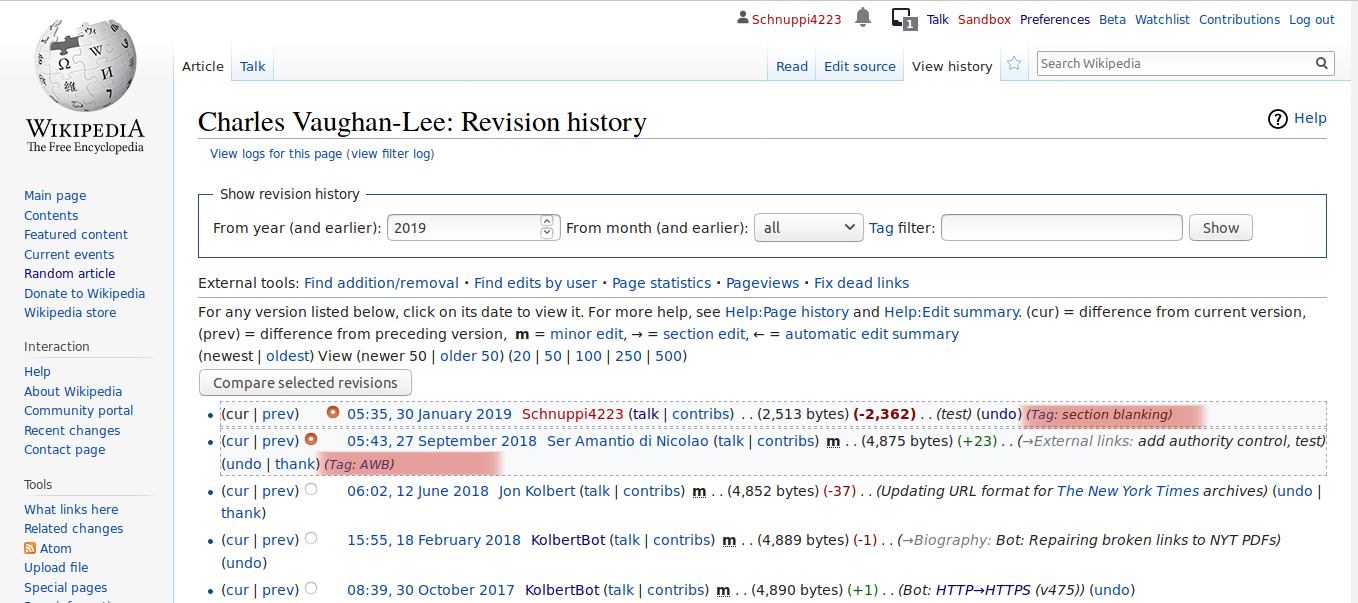
\includegraphics[width=0.9\columnwidth]{figures/screenshots-filter-trigger/Screenshot-tags-in-revision-history.png}
  \caption{Tagged edits are marked as such in a page's revision history}~\label{fig:tags-in-history}
\end{figure}

\begin{figure}
\centering
  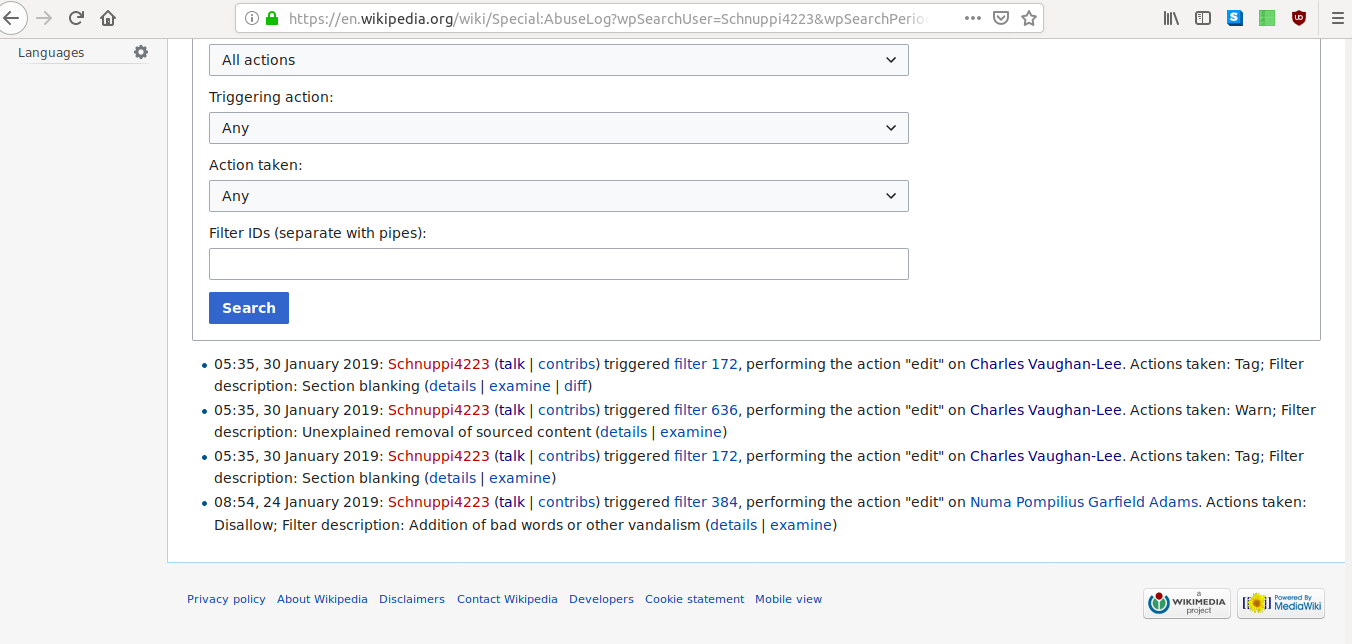
\includegraphics[width=0.9\columnwidth]{figures/screenshots-filter-trigger/Screenshot-abuse-log.png}
  \caption{Abuse Log showing all filter triggers by User Schnuppi4223}~\label{fig:screenshot-abuse-log}
\end{figure}

If the filter is set to disallow, a specific template is shown to the editor: "An automated filter has identified this edit as potentially unconstructive, so it has been disallowed. If this edit is constructive, please report this error. Disruptive editing may result in a block from editing."
"report this error" links to the FalsePositives page: \url{https://en.wikipedia.org/wiki/Wikipedia:Edit_filter/False_positives}
"block from editing" links to \url{https://en.wikipedia.org/wiki/Wikipedia:Blocking_policy}

The edit is not saved.

So far, I haven't managed to trigger a filter with a different action.

\begin{figure}
\centering
  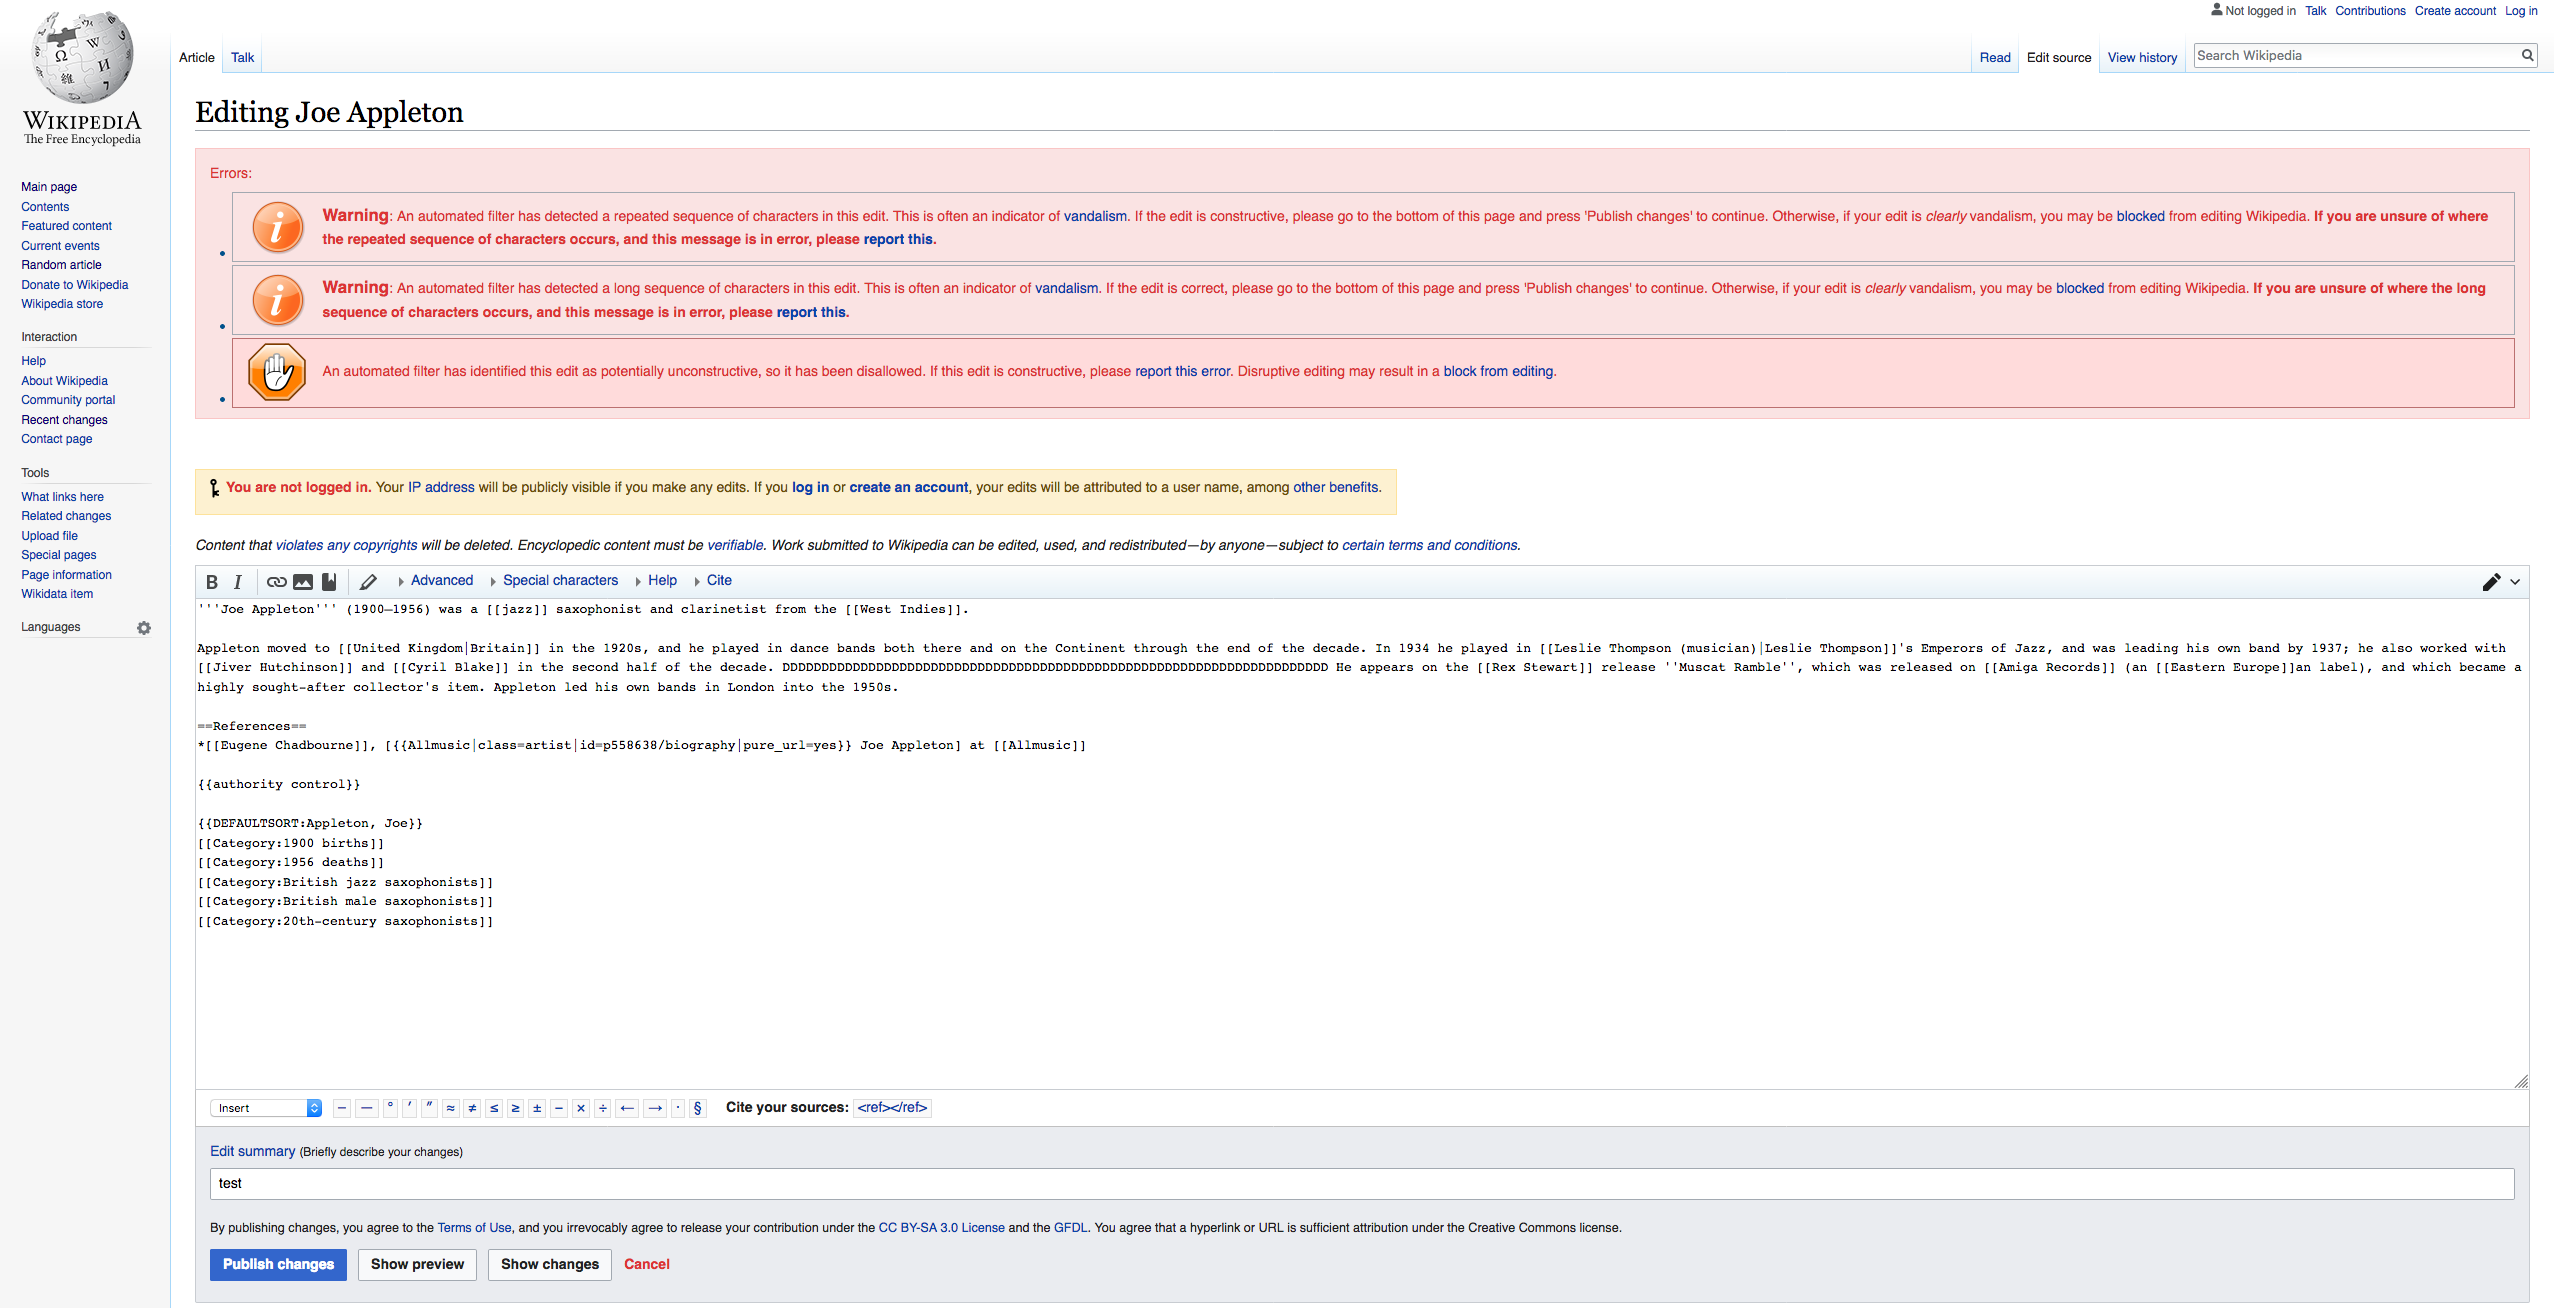
\includegraphics[width=0.9\columnwidth]{figures/screenshots-filter-trigger/Screenshot-trigger-warning-filter.png}
  \caption{Editor gets notified their edit triggered multiple edit filters}~\label{fig:screenshot-warn-disallow}
\end{figure}

\subsection{TOR}
(Interesting side note: editing via TOR is disallowed: "Your IP has been recognised as a TOR exit node. We disallow this to prevent abuse" or similar, check again for wording. Compare: "Users of the Tor anonymity network will show the IP address of a Tor "exit node". Lists of known Tor exit nodes are available from the Tor Project's Tor Bulk Exit List exporting tool." \url{https://en.wikipedia.org/wiki/Wikipedia:Vandalism})



\section{Edit filters on the English Wikipedia: State of the art}

\textbf{Interesting questions}
\begin{itemize}
    \item how many filters are there (were there over the years): 954 filters (stand: 06.01.2019); TODO: historically?
    \item what do the most active filters do?: see~\ref{tab:most-active-actions}
    \item get a sense of what gets filtered (more qualitative): TODO: refine after sorting through manual categories; preliminary: vandalism; unintentional suboptimal behavior from new users who don't know better ("good faith edits") such as blanking an article/section; creating an article without categories; adding larger texts without references; large unwikified new article (180); or from users who are too lazy (to write proper edit summaries; editing behaviours and styles not suitable for an encyclopedia (poor grammar/not commiting to orthography norms; use of emoticons and !; ascii art?); "unexplained removal of sourced content" (636) may be an attempt to silence a view point the editor doesn't like; self-promotion(adding unreferenced material to BLP; "users creating autobiographies" 148;); harassment; sockpuppetry; potential copyright violations; that's more or less it actually. There's a third bigger cluster of maintenance stuff, such as tracking bugs or other problems, trying to sort through bot edits and such. For further details see the jupyter notebook.
    \item has the willingness of the community to use filters increased over time?: looking at aggregated values of number of triggered filters per year, the answer is rather it's quite constant; TODO: plot it at a finer granularity
    \item how often were (which) filters triggered: see \url{filter-lists/20190106115600_filters-sorted-by-hits.csv} and~\ref{tab:most-active-actions}; see also jupyter notebook for aggregated hitcounts over tagged categories
    \item percentage of triggered filters/all edits; break down triggered filters according to typology: TODO still need the complete abuse\_filter\_log table!; and probably further dumps in order to know total number of edits
    \item percentage filters of different types over the years: TODO according to actions (I need a complete abuse\_filter\_log table for this!); according to self-assigned tags (finish tagging!)
    \item what gets classified as vandalism? has this changed over time? TODO: (look at words and patterns triggered by the vandalism filters; read vandalism policy page); pay special attention to filters labeled as vandalism by the edit filter editors (i.e. in the public description) vs these I labeled as vandalism
\end{itemize}

\textbf{Questions on abuse\_filter table}
\begin{itemize}
    \item how many filters are there altogether
    \item how many are enabled/disabled?
    \item how many hidden filters? how many of them are enabled
    \item how many are marked as deleted? (how many of them are hidden?)
    \item how many global? (what does global mean?)
    \item how many throttled? (what does this mean?)
    \item how many currently trigger which action (disallow, warn, throttle, tag, ..)?
    \item explore timestamp (I think it means "last modified"): have a lot of filters been modified recently?
    \item what are the values in the "group" column? what do they mean?
    \item which are the most frequently triggered filters of all time?
    \item is it new filters that get triggered most frequently? or are there also very active old ones?
    \item how many different edit filter editors are there (af\_user)?
    \item categorise filters according to which name spaces they apply to; pay special attention to edits in user/talks name spaces (may be indication of filtering harassment)
\end{itemize}

\textbf{Questions on abuse\_filter\_log table}
\begin{itemize}
    \item how often were filters with different actions triggered? (afl\_actions)
    \item what types of users trigger the filters (IPs? registered?)
    \item on what articles filters get triggered most frequently (afl\_title)
    \item what types of user actions trigger filters most frequently? (afl\_action) (edit, delete, createaccount, move, upload, autocreateaccount, stashupload)
    \item in which namespaces get filters triggered most frequently?
\end{itemize}

\textbf{Questions on abuse\_filter\_action table}
\begin{itemize}
    \item how many filters trigger any particular action (at the moment)?
    \item how many different parameters are there (i.e. tags when tagging, or templates to show upon a warning)?
\end{itemize}

\textbf{Number of unique filters that were triggered each year since 2009:}
owing to quarries we have all the filters that were triggered from the filter log per year, from 2009 (when filters were first introduced/the MediaWiki extension was enabled) till end of 2018 with their corresponding number of times being triggered:
\begin{table}
  \centering
  \begin{tabular}{l r }
    % \toprule
    Year & Num of distinct filters \\
    \hline
    2009 & 220 \\
    2010 & 163 \\
    2011 & 161 \\
    2012 & 170 \\
    2013 & 178 \\
    2014 & 154 \\
    2015 & 200 \\
    2016 & 204 \\
    2017 & 231 \\
    2018 & 254 \\
    % \bottomrule
  \end{tabular}
  \caption{Count of distinct filters that got triggered each year}~\label{tab:active-filters-count}
\end{table}

data is still not enough for us to talk about a tendency towards introducing more filters (after the initial dip)


\textbf{Most frequently triggered filters for each year:}
10 most active filters per year:
\begin{table}
  \centering
  \begin{tabular}{r r }
    % \toprule
    Filter ID & Hitcount \\
    \hline
    135 & 175455 \\
    30 & 160302 \\
    61 & 147377 \\
    18 & 133640 \\
    3 & 95916 \\
    172 & 89710 \\
    50 & 88827 \\
    98 & 80434 \\
    65 & 74098 \\
    132 & 68607 \\
    % \bottomrule
  \end{tabular}
  \caption{10 most active filters in 2009}~\label{tab:most-active-2009}
\end{table}

\begin{table}
  \centering
  \begin{tabular}{r r }
    % \toprule
    Filter ID & Hitcount \\
    \hline
    61 & 245179 \\
    135 & 242018 \\
    172 & 148053 \\
    30 & 119226 \\
    225 & 109912 \\
    3 & 105376 \\
    50 & 101542 \\
    132 & 78633 \\
    189 & 74528 \\
    98 & 54805 \\
    % \bottomrule
  \end{tabular}
  \caption{10 most active filters in 2010}~\label{tab:most-active-2010}
\end{table}

\begin{table}
  \centering
  \begin{tabular}{r r }
    % \toprule
    Filter ID & Hitcount \\
    \hline
    61 & 218493 \\
    135 & 185304 \\
    172 & 119532 \\
    402 & 109347 \\
    30 & 89151 \\
    3 & 75761 \\
    384 & 71911 \\
    225 & 68318 \\
    50 & 67425 \\
    432 & 66480 \\
    % \bottomrule
  \end{tabular}
  \caption{10 most active filters in 2011}~\label{tab:most-active-2011}
\end{table}

\begin{table}
  \centering
  \begin{tabular}{r r }
    % \toprule
    Filter ID & Hitcount \\
    \hline
    135 & 173830 \\
    384 & 144202 \\
    432 & 126156 \\
    172 & 105082 \\
    30 & 93718 \\
    3 & 90724 \\
    380 & 67814 \\
    351 & 59226 \\
    279 & 58853 \\
    225 & 58352 \\
    % \bottomrule
  \end{tabular}
  \caption{10 most active filters in 2012}~\label{tab:most-active-2012}
\end{table}

\begin{table}
  \centering
  \begin{tabular}{r r }
    % \toprule
    Filter ID & Hitcount \\
    \hline
    135 & 133309 \\
    384 & 129807 \\
    432 & 94017 \\
    172 & 92871 \\
    30 & 85722 \\
    279 & 76738 \\
    3 & 70067 \\
    380 & 58668 \\
    491 & 55454 \\
    225 & 48390 \\
    % \bottomrule
  \end{tabular}
  \caption{10 most active filters in 2013}~\label{tab:most-active-2013}
\end{table}

\begin{table}
  \centering
  \begin{tabular}{r r }
    % \toprule
    Filter ID & Hitcount \\
    \hline
    384 & 111570 \\
    135 & 111173 \\
    279 & 97204 \\
    172 & 82042 \\
    432 & 75839 \\
    30 & 62495 \\
    3 & 60656 \\
    636 & 52639 \\
    231 & 39693 \\
    380 & 39624 \\
    % \bottomrule
  \end{tabular}
  \caption{10 most active filters in 2014}~\label{tab:most-active-2014}
\end{table}

\begin{table}
  \centering
  \begin{tabular}{r r }
    % \toprule
    Filter ID & Hitcount \\
    \hline
    650 & 226460 \\
    61 & 196986 \\
    636 & 191320 \\
    527 & 189911 \\
    633 & 162319 \\
    384 & 141534 \\
    279 & 110137 \\
    135 & 99057 \\
    686 & 95356 \\
    172 & 82874 \\
    % \bottomrule
  \end{tabular}
  \caption{10 most active filters in 2015}~\label{tab:most-active-2015}
\end{table}

\begin{table}
  \centering
  \begin{tabular}{r r }
    % \toprule
    Filter ID & Hitcount \\
    \hline
    527 & 437099 \\
    61 & 274945 \\
    650 & 229083 \\
    633 & 218696 \\
    636 & 179948 \\
    384 & 179871 \\
    279 & 106699 \\
    135 & 95131 \\
    172 & 79843 \\
    30 & 68968 \\
    % \bottomrule
  \end{tabular}
  \caption{10 most active filters in 2016}~\label{tab:most-active-2016}
\end{table}

\begin{table}
  \centering
  \begin{tabular}{r r }
    % \toprule
    Filter ID & Hitcount \\
    \hline
    61 & 250394 \\
    633 & 218146 \\
    384 & 200748 \\
    527 & 192441 \\
    636 & 156409 \\
    650 & 151604 \\
    135 & 80056 \\
    172 & 70837 \\
    712 & 59537 \\
    833 & 58133 \\
    % \bottomrule
  \end{tabular}
  \caption{10 most active filters in 2017}~\label{tab:most-active-2017}
\end{table}

\begin{table}
  \centering
  \begin{tabular}{r r }
    % \toprule
    Filter ID & Hitcount \\
    \hline
    527 & 358210 \\
    61 & 234867 \\
    633 & 201400 \\
    384 & 177543 \\
    833 & 161030 \\
    636 & 144674 \\
    650 & 79381 \\
    135 & 75348 \\
    686 & 70550 \\
    172 & 64266 \\
    % \bottomrule
  \end{tabular}
  \caption{10 most active filters in 2018}~\label{tab:most-active-2018}
\end{table}

\textbf{what do the most active filters do?}

\begin{table*}
  \centering
    \begin{tabular}{r p{10cm} p{5cm} }
    % \toprule
    Filter ID & Publicly available description & Actions \\
    \hline
      135 & repeating characters & tag, warn \\
      30 & "large deletion from article by new editors" & tag, warn \\
      61 & "new user removing references" ("new user" is handled by "!("confirmed" in user\_groups)") & tag \\
      18 & "test type edits from clicking on edit bar" (people don't replace Example texts when click-editing) & deleted in Feb 2012 \\
      3 & "new user blanking articles" & tag, warn \\
      172 & "section blanking" & tag \\
      50 & "shouting" (contribution consists of all caps, numbers and punctuation) & tag, warn \\
      98 & "creating very short new article" & tag \\
      65 & "excessive whitespace" (note: "associated with ascii art and some types of vandalism") & deleted in Jan 2010 \\
      132 & "removal of all categories" & tag, warn \\
      225 & "vandalism in all caps" (difference to 50? seems to be swear words, but shouldn't they be catched by 50 anyway?) & disallow \\
      189 & "BLP vandalism or libel" & tag \\
      402 & "new article without references" & deleted in Apr 2013, before that disabled with comment "disabling, no real use" \\
      384 & "addition of bad words or other vandalism" (seems to be a blacklist) & disallow \\
      432 & "starting new line with lower case letters" & tag, warn //I recall there was a rule of thumb recommending not to user filters for style things? although that's not really style, but rather wrong grammar.. \\
      380 & hidden; public comment "multiple obscenities" & disallow \\
      351 & "text added after categories and interwiki" & tag, warn \\
      279 & "repeated attempts to vandalise" & tag, throttle (triggered when someone hits "edit" repeatedly in a short ammount of time) \\
      491 & "edits ending with emoticons or !" & tag, warn \\
      636 & "unexplained removal of sourced content" & warn (that, together with 634 and 635 refutes my theory that warn always goes together with tag) \\
      231 & "long string of characters containing no spaces" (that's surely english though^^) & tag, warn \\
      650 & "creation of a new article without any categories" & (log only) \\
      527 & hidden; public comments "T34234: log/throttle possible sleeper account creations" & throttle \\
      633 & "possible canned edit summary" (apparently pre-filled on mobile though) & tag \\
      686 & "IP adding possible unreferenced material to BLP" (BLP= biography of living people? I thought, it was forbidden to edit them without a registered account) & (log only) \\
      712 & "possibly changing date of birth in infobox" ("possibly"? and I thought infoboxes were pre-generated from wikidata?) & (log only) \\
      833 & "newer user possibly adding a unreferenced or improperly referenced material" & (log only) \\
  \end{tabular}
  \caption{What do most active filters do?}~\label{tab:most-active-actions}
\end{table*}

\subsection{Types of edit filters}

\textbf{Hidden filters}
\url{https://en.wikipedia.org/wiki/Wikipedia:Edit_filter}
"Non-admins in good standing who wish to review a proposed but hidden filter may message the mailing list for details."
// what is "good standing"?
// what are the arguments for hiding a filter? --> particularly obnoctious vandals can see how their edits are being filtered and circumvent them; security through obscurity
"Filters should only be hidden where necessary, such as in long-term abuse cases where the targeted user(s) could review a public filter and use that knowledge to circumvent it. Filters should not generally be named after abusive editors, but rather with a simple description of the type of abuse, provided not too much information is given away."
// are users still informed if their edit triggers a hidden filter?

"For all filters, including those hidden from public view, a brief description of what the rule targets is displayed in the log, the list of active filters, and in any error messages generated by the filter. "

"Be careful not to test sensitive parts of private filters in a public test filter (such as Filter 1): use a private test filter (for example Filter 2) if testing is required."

harassment! mailinglist
"If it would not be desirable to discuss the need for a given edit filter on-wiki, such as where the purpose of the filter is to combat harassment by an abusive banned user who is likely to come across the details of the request, edit filter managers can be emailed directly or on the wikipedia-en-editfilters mailing list at wikipedia-en-editfilters@lists.wikimedia.org."

\url{https://lists.wikimedia.org/mailman/listinfo/wikipedia-en-editfilters}
"private mailing list used by English Wikipedia edit filter managers, "
"primarily for discussing hidden filters."
"The mailing list should not be used as a venue for discussions that could reasonably be held on-wiki."

There's also separate documentation of long term abuse (see notes)


\section{Critical discussion}

* why get certain filters (and not others?)
* do filter solve effectively the task they were conjured up to life to fulfil?
* what kinds of biases/problems are there?
* who is allowed to edit edit filters?

\section{Conclusion}

It is important that you write for the SIGCHI audience. Please read
previous years' proceedings to understand the writing style and
conventions that successful authors have used. It is particularly
important that you state clearly what you have done, not merely what
you plan to do, and explain how your work is different from previously
published work, i.e., the unique contribution that your work makes to
the field. Please consider what the reader will learn from your
submission, and how they will find your work useful. If you write with
these questions in mind, your work is more likely to be successful,
both in being accepted into the conference, and in influencing the
work of our field.

\section{Acknowledgments}

Sample text: We thank all the volunteers, and all publications support
and staff, who wrote and provided helpful comments on previous
versions of this document. Authors 1, 2, and 3 gratefully acknowledge
the grant from NSF (\#1234--2012--ABC). \textit{This whole paragraph is
  just an example.}

% Balancing columns in a ref list is a bit of a pain because you
% either use a hack like flushend or balance, or manually insert
% a column break.  http://www.tex.ac.uk/cgi-bin/texfaq2html?label=balance
% multicols doesn't work because we're already in two-column mode,
% and flushend isn't awesome, so I choose balance.  See this
% for more info: http://cs.brown.edu/system/software/latex/doc/balance.pdf
%
% Note that in a perfect world balance wants to be in the first
% column of the last page.
%
% If balance doesn't work for you, you can remove that and
% hard-code a column break into the bbl file right before you
% submit:
%
% http://stackoverflow.com/questions/2149854/how-to-manually-equalize-columns-
% in-an-ieee-paper-if-using-bibtex
%
% Or, just remove \balance and give up on balancing the last page.
%
\balance{}

% BALANCE COLUMNS
\balance{}

% REFERENCES FORMAT
% References must be the same font size as other body text.
\bibliographystyle{SIGCHI-Reference-Format}
\bibliography{literature}

\end{document}

%%% Local Variables:
%%% mode: latex
%%% TeX-master: t
%%% End:
